\documentclass[a4 paper]{article}
%\usepackage{minted}           %embedding code
\usepackage{amsmath, amsthm, amsfonts} %always use amsmath for symbols, amsthm for theorems 
\usepackage{graphicx}  % for pictures
%\usepackage{lipsum}  % for test text
\usepackage{multicol}    % for multicollumn text
\usepackage[bottom=2.5cm]{geometry}   %to set the margins to your liking
\usepackage[skip = 10pt, indent = 30pt]{parskip}      %to set the distance between paragraphs
\usepackage{tcolorbox}           %for literal color boxes
%\usepackage{witharrows}             % understandable, arrows for equations
\usepackage{tikz}                   %drawings and diagrams
\usetikzlibrary{positioning}        %tikz library for positioning (of nodes?)
\usepackage{pgfplots}               %plotting and graphs
\pgfplotsset{compat=1.18, width = 10cm}
\usepackage{hyperref}
\hypersetup{colorlinks = true, linkcolor = black, urlcolor = blue}
%\usepackage{fancyvrb}           % fancy formatting of verbatim
%\usepackage{fancyhdr, lastpage}
%\pagestyle{fancy} 
%\lhead{Relat\'orio experimento 4}
%\rhead{FisExpI}
%\cfoot{Página \thepage \ de \pageref{LastPage}}
%\usepackage[Bjornstrup]{fncychap} %Sonny, Glenn, Lenny, Conny, Rejne, Bjarne, Bjornstrup
%\usepackage{xcolor}      %color text
\usepackage{siunitx}    %for SI units
\usepackage{setspace}
\onehalfspacing
\usepackage{cleveref}
\usepackage[brazil]{babel}
\usepackage{caption}
\usepackage{subcaption}
\usepackage{pdfpages}
\usepackage{booktabs}
\usepackage{multirow}
\usepackage{textcomp}
\usepackage{amssymb}
\usepackage[document]{ragged2e}
\usepackage{bm}
\usepackage{empheq}




%\setlength{\hoffset}{-2cm}
%\setlength{\voffset}{1.5cm}                     %control your margins however you want!
%\setlength{\marginparwidth}{2cm}
%\setlength{\oddsidemargin}{0cm}

%\newtheorem{theorem}{Theorem}[section]               %how you call it and how you display it
%\newtheorem{corollary}{Corollary}[theorem]


\newcommand{\parag}{\hspace{30pt}}
%\newcommand{\pd}[2]{\frac{\partial#1}{\partial#2}}


\begin{document}
\justifying
\begin{center}{\large Laboratório de Circuitos Elétricos - 02/2024 - Turma 05}\\
{\large \textbf{Experimento 3}}\\ 
14/11/2024
\end{center}

\vspace{500pt}
 \noindent\textbf{Grupo 5:}\\
 Yuri Shumyatsky - 231012826\\
Vinicius de Melo Moraes - 231036274


\vspace{30pt}
\newpage

\section{Introdução}
\parag O experimento de Teoremas de Circuitos tem como objetivo explorar e comprovar a aplicação de teoremas fundamentais na análise de circuitos elétricos. No decorrer das atividades experimentais, são utilizados componentes como resistores, fontes de tensão e equipamentos de medição para observar o comportamento de circuitos simples e complexos. Os teoremas abordados incluem o de superposição, Thévenin e Norton, permitindo que seja adquirida uma compreensão prática da simplificação e análise de circuitos. Por meio da montagem e medição de tensões, correntes e resistências, o experimento visa consolidar o conhecimento teórico sobre como esses teoremas podem ser aplicados para prever e calcular parâmetros em circuitos reais.


\section{Materiais}
\begin{itemize}
\item Multímetro - Agilent 34410A
\item Fonte DC - Agilent E3631A
\item Protoboard
\item Década resistiva
\item 1 resistor de 1,5k$\Omega$
\item 1 resistor de 1,2k$\Omega$
\item 1 resistor de 1k$\Omega$
\item 1 resistor de 1,8k$\Omega$
\item 1 resistor de 2,2k$\Omega$
\end{itemize}


 Para o grupo 5, foi definido que $R_1=1,2k\Omega, R_2=1,5k\Omega, R_3=1,8k\Omega,$ $R_4=2,2k\Omega, R_5=1k\Omega, V_{S1}=3V, V_{S2}=2V$.

A configuração inicial do circuito é:

\begin{table}[h]
\centering
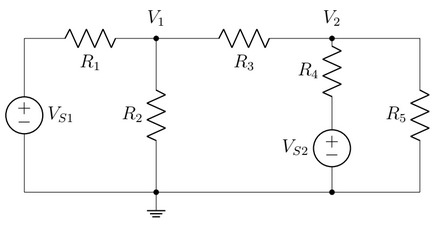
\includegraphics[scale=0.6]{figuras/figura1}
\end{table}

\begin{center}
Figura 1: Circuito inicial
\end{center}


\newpage\section{Experimento}

\parag Como usual, as resistências são medidas e comparadas com os valores teóricos, de forma a preencher a Tabela 1.

\vspace{5pt}
\begin{table}[h]
\centering
\begin{tabular}{|c|c|c|c|}
\hline
 Resistência & Valor nominal & Valor medido & Erro (\%) \\\hline
 $R_1$&$1,2\cdot10^3\Omega$ &$1,179\cdot10^3\Omega$ &1,75 \\\hline
 $R_2$&$1,5\cdot10^3\Omega$ &$1,495\cdot10^3\Omega$ &0,33 \\\hline
 $R_3$&$1,8\cdot10^3\Omega$ &$1,822\cdot10^3\Omega$ &1,22 \\\hline
 $R_4$&$2,2\cdot10^3\Omega$ &$2,181\cdot10^3\Omega$ &0,86 \\\hline
 $R_5$&$1\cdot10^3\Omega$ &$0,990\cdot10^3\Omega$ &1,00 \\\hline
\end{tabular}
\caption*{Tabela 1: Resistências}
\end{table}

Em seguida, já com o circuito montado, são medidas as tensões relevantes. Para calcular os valores de $V_1$ e $V_2$, é usada a seguinte análise nodal:

\noindent Nó 1:
\[\frac{V_2-V_1}{1,8\cdot10^3}+\frac{0-V_1}{1,5\cdot10^3}+\frac{3-V_1}{1,2\cdot10^3}=0 \implies \frac{V_2-3,7V_1+4,5}{1,8}=0 \implies V_2-3,7V_1+4,5=0\]

\noindent Nó 2:
\[\frac{-(V_2-V_1)}{1,8\cdot10^3}+\frac{2-V_2}{2,2\cdot10^3}+\frac{0-V_1}{1\cdot10^3}=0\implies \frac{-2,2V_2-7,96V_2+3,6}{3,96}\implies-2,2V_2-7,96V_2+3,6=0 \]

\noindent O que nos dá o seguinte sistema:
\begin{equation*}
\left\{
\begin{aligned}
V_2-3,7V_1+4,5=0  \\
2,2V_1-7,96V_2+3,6=0
\end{aligned}\right.
\end{equation*}

\noindent que usamos na forma matricial e realizamos a eliminação de Gauss-Jordan para resolver. A forma matricial é dada por A e a matriz equivalente pós Gauss-Jordan é dada por A'.

\[
A=
\begin{bmatrix}
-3,7 & 1 & -4,5\\
2,2 & -7,96 & 3,6
\end{bmatrix},\ \ 
A'=
\begin{bmatrix}
-3,7 & 1 & -4,5\\
0 & -7,37 & -6,64
\end{bmatrix}
\]

\noindent Do sistema equivalente a A',

\begin{equation*}
\left\{
\begin{aligned}
-3,7V_1+V_2=4,5\\
	-7,37V_2=6,64
\end{aligned}\right.
\end{equation*}

\noindent é fácil ver que $V_1=1,46$ e $V_2=0,901$

\vspace{5pt}
\begin{table}[h]
\centering
\begin{tabular}{|c|c|c|c|}
\hline
Tensão & Valor Calculado (V) & Valor Medido (V) & Erro (\%) \\\hline
$V_1$ & $1,460$&1,455 &0,34 \\\hline
$V_2$ & 0,901&0,851 &5,55 \\\hline
$V_{S1}$ &3 &2,979 &0,70 \\\hline
$V_{S2}$ & 2&2,000 &0,00 \\\hline
\end{tabular}
\caption*{Tabela 2: Tensões}
\end{table}



\newpage Tendo essas informações, a fonte $V_{S1}$ é substituída por um fio e são medidas e calculadas as tensões nodais para os nós 1 e 2.
O cálculo para encontrar as tensões nodais é análogo ao que foi feito previamente e resulta no sistema representado pela matriz B:

\[B=
\begin{bmatrix}
-3,7 & 1 & 0\\
2,2 & -7,56 & -3,6
\end{bmatrix}
\]

\noindent que é reduzido a
\[
B'=
\begin{bmatrix}
-3,7 & 1 & 0\\
0 & -7,37 & -3,6 
\end{bmatrix}
\]

\noindent de onde segue que $V_{1a}=0,132$ e $V_{2a}=0,488$


\vspace{5pt}
\begin{table}[h]
\centering
\begin{tabular}{|c|c|c|c|}
\hline
 Tensão & Valor Calculado (V) & Valor Medido (V) & Erro(\%) \\\hline
$V_{1a}$ & 0,132 & 0,130 & 1,52 \\\hline
$V_{2a}$ & 0,488 & 0,490 & 0,41\\\hline
\end{tabular}
\caption*{Tabela 3: Tensões sem a fonte $V_{S1}$}
\end{table}

O mesmo processo é feito ao substituir $V_{S2}$ em vez de $V_{S1}$ e obtemos, de forma análoga, o sistema representado pela matriz C e sua versão reduzida em C':

\[
C=
\begin{bmatrix}
-3,7&1&-4,5\\
2,2&-7,96&0
\end{bmatrix},\ \ 
C'=
\begin{bmatrix}
-3,7&1&-4,5\\
0&-7,37&2,68
\end{bmatrix}
\]

\noindent de onde segue que $V_{1b}=0,132$ e $V_{2b}=0,488$

\vspace{5pt}
\begin{table}[h]
\centering
\begin{tabular}{|c|c|c|c|}
\hline
Tensão & Valor Calculado (V) & Valor Medido (V) & Erro (\%) \\\hline
 $V_{1b}$&1,314 &1,328 & 1,06\\\hline
 $V_{2b}$&0,363 &0,359 &1,10 \\\hline
\end{tabular}
\caption*{Tabela 4: Tensões sem $V_{S2}$}
\end{table}

\newpage Para verificar o princípio de superposição, usando os valores encontrados anteriormente:

\vspace{5pt}
\begin{table}[h]
\centering
\begin{tabular}{|c|c|c|c|}
\hline
 Tensão&Valor Calculado (V) & Valor Medido (V) & Erro (\%) \\\hline
$V_{1a}+V_{1b}$ &1,446 &1,458 &0,83 \\\hline
$V_{2a}+V_{2b}$ &0,851 &0,849 &0,24 \\\hline
\end{tabular}
\caption*{Tabela 5: Superposição}
\end{table}

Em seguida, $R_5$ é substituída por um fio, de forma a realizar um curto circuito cuja corrente será medida, depois será feita a medição da tensão de circuito aberto e da resistência equivalente na mesma posição.  

Para encontrar a corrente de curto circuito, é feita a análise de malhas:

\begin{equation*}
\left\{
\begin{aligned}
-3+1,2\cdot10^3I_1+1,5\cdot10^3(I_1-I_2)=0\hspace{20pt}(Malha\ 1)\\
2+1,8\cdot10^3I_2+1,5\cdot10^3(I_2-I_1)+2,2\cdot10^3(I_2-I_3)=0\hspace{20pt}(Malha\ 2)\\
-2+2,2\cdot10^3(I_3-I_2)=0\hspace{20pt}(Malha\ 3)
\end{aligned}
\right.
\end{equation*}

\noindent que após simplificar e colocar na forma matricial obtemos a matriz D, que é reduzida via eliminação de Gauss-Jordan para a matriz D':

\[
D=
\begin{bmatrix}
2,7 & -1,5 & 0 & 3\\
-1,5 & 5,5 & -2,2 & -2\\
0 & -2,2 & 2,2 & 2
\end{bmatrix}, \ \ 
D'=
\begin{bmatrix}
2,7 & -1,5 & 0 & 3\\
0 & 4,67 & -2,2 & -0,33\\
0 & 0 & 1,16 & 1,84
\end{bmatrix}
\]

\noindent de onde segue que $1,16I_3 = 1,84 \implies I_3 = I_{SC} = 1,59$

Para encontrar $V_{OC}$, usa-se a análise nodal, que de forma análoga às outras análises feitas previamente resulta no seguinte sistema:


Nó 1:
\[
\frac{3-V_1}{1,2\cdot10^3}+\frac{0-V_1}{1,5\cdot10^3}+\frac{V_2-V_1}{1,8\cdot10^3}=0 \implies 4,5-3,7V_1+V_2=0
\]

Nó 2:
\[
\frac{2-V_2}{2,2\cdot10^3}-\frac{(V_2-V_1)}{1,8\cdot10^3}=0 \implies 3,6-4V_2+2,2V_1=0
\]

\noindent que na forma matricial resulta na matriz E e sua forma simplificada E':

\[
E=
\begin{bmatrix}
-3,7 & 1 & -4,5\\
2,2 & -4 & -3,6
\end{bmatrix},\ \ 
E' =
\begin{bmatrix}
-3,7 & 1 & -4,5\\
0 & -3,41 & -6,2
\end{bmatrix}
\]

\noindent de onde segue facilmente que $-3,41V_2=-6,2 \implies V_2 = V_{OC}= 1,843V$.

Por fim, o cálculo da $R_{eq}$ é simplesmente $R_{eq}=((R_1//R_2)+R_3)//R_4=1,163k\Omega$

\vspace{5pt}
\begin{table}[h]
\centering
\begin{tabular}{|c|c|c|c|}
\hline
 Grandeza & Valor Calculado & Valor Medido & Erro (\%) \\\hline
 $I_{SC}$ &1,590mA &1,584mA & 0,38\\\hline
 $V_{OC}$& 1,821V & 1,843V & 1,19 \\\hline
 $R_{eq}$&1,163k$\Omega$ &1,161k$\Omega$ & 0,17 \\\hline
 ${V_{OC}}/{I_{SC}}$&1,145k$\Omega$ &1,164k$\Omega$ &1,62 \\\hline
\end{tabular}
\caption*{Tabela 6: Corrente de curto-circuito, tensão de circuito aberto e resistência equivalente}
\end{table}


Usando os valores encontrados anteriormente, foi montado o circuito equivalente de Thévenin, da forma da Figura 2.

\begin{table}[h]
\centering
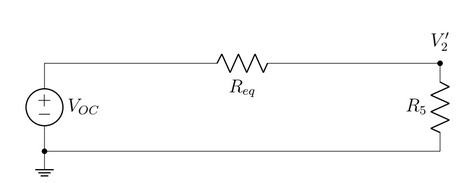
\includegraphics[scale=0.6]{figuras/figura2}
\end{table}
\begin{center}
Figura 2: Circuito de Thévenin
\end{center}

Os valores calculados de $V_{OC}$ e de $R_{eq}$ são os mesmos medidos da Tabela 6. Para encontrar $V_2'$, é feita a seguinte análise nodal:

\[
\frac{1,84-V_2'}{1,2\cdot10^3} + \frac{0-V_2'}{1\cdot10^3}=0 \implies 1,84-2,2V_2'=0 \implies V_2'=0,836V
\] 

\vspace{5pt}
\begin{table}[h]
\centering
\begin{tabular}{|c|c|c|c|}
\hline
 Grandeza & Valor Calculado & Valor Medido & Erro (\%) \\\hline
$V_{OC}$ & 1,843V & 1,842V &0,05 \\\hline
$R_{eq}$ & 1,161k$\Omega$ &  1,161k$\Omega$ & 0,00\\\hline
$V_2'$ & 0,836V & 0,843V &0,84 \\\hline
\end{tabular}
\caption*{Tabela 7: Circuito de Thévenin}
\end{table}

\newpage
\section{Conclusão}

\parag O estudo e a aplicação prática dos teoremas de Thévenin, Norton e da sobreposição demonstraram a eficácia dessas ferramentas na análise e simplificação de circuitos elétricos complexos. A utilização do circuito equivalente de Thévenin permitiu prever com precisão o comportamento do sistema, enquanto o princípio da sobreposição facilitou a análise de circuitos lineares com múltiplas fontes. Os resultados experimentais confirmaram a validade dos métodos teóricos, evidenciando sua relevância na engenharia elétrica para a resolução eficiente de problemas e otimização de sistemas elétricos.

\vspace{80pt}
\section{Bibliografia}
\begin{itemize}
\item HALLIDAY, D.; RESNICK, R.; WALKER, J. Fundamentos de Física. 10. ed. v. 3. Rio de Janeiro: LTC, 2016.
\end{itemize}







\end{document}